\documentclass{beamer}

\mode<presentation> {

%\usetheme{default}
%\usetheme{AnnArbor}
%\usetheme{Antibes}
%\usetheme{Bergen}
%\usetheme{Berkeley}
%\usetheme{Berlin}
%\usetheme{Boadilla}
%\usetheme{CambridgeUS}
%\usetheme{Copenhagen}
%\usetheme{Darmstadt}
%\usetheme{Dresden}
%\usetheme{Frankfurt}
%\usetheme{Goettingen}
%\usetheme{Hannover}
%\usetheme{Ilmenau}
%\usetheme{JuanLesPins}
%\usetheme{Luebeck}
\usetheme{Madrid}
%\usetheme{Malmoe}
%\usetheme{Marburg}
%\usetheme{Montpellier}
%\usetheme{PaloAlto}
%\usetheme{Pittsburgh}
%\usetheme{Rochester}
%\usetheme{Singapore}
%\usetheme{Szeged}
%\usetheme{Warsaw}


%\usecolortheme{albatross}
%\usecolortheme{beaver}
%\usecolortheme{beetle}
%\usecolortheme{crane}
%\usecolortheme{dolphin}
%\usecolortheme{dove}
%\usecolortheme{fly}
%\usecolortheme{lily}
%\usecolortheme{orchid}
%\usecolortheme{rose}
%\usecolortheme{seagull}
%\usecolortheme{seahorse}
%\usecolortheme{whale}
%\usecolortheme{wolverine}

%\setbeamertemplate{footline} % To remove the footer line in all slides uncomment this line
%\setbeamertemplate{footline}[page number] % To replace the footer line in all slides with a simple slide count uncomment this line

%\setbeamertemplate{navigation symbols}{} % To remove the navigation symbols from the bottom of all slides uncomment this line
}

\usepackage{graphicx} % Allows including images
\usepackage{booktabs} % Allows the use of \toprule, \midrule and \bottomrule in tables
\usepackage{amsfonts}
\usepackage{mathrsfs, bbold}
\usepackage{amsmath,amssymb,graphicx}

%----------------------------------------------------------------------------------------
%	TITLE PAGE
%----------------------------------------------------------------------------------------

\title["2"]{2: Single-parameter models}

% \author{Taylor} 
% \institute[UVA] 
% {
% University of Virginia \\
% \medskip
% \textit{} 
% }
\date{08/28/19} 

\begin{document}
%----------------------------------------------------------------------------------------

\begin{frame}
\titlepage 
\end{frame}

\section{2.1}

%----------------------------------------------------------------------------------------
\begin{frame}
\frametitle{Introduction}

We discuss prior selection, and demonstrate new ideas with examples of models with only one parameter.


\end{frame}

%----------------------------------------------------------------------------------------


\begin{frame}
\frametitle{Binomial: from prior to posterior}

Let $y$ be the number of $n$ births that are female. Let $\theta$ be the population proportion of births that are female 
\newline

Likelihood:
\begin{enumerate}
\item $y \mid \theta \sim \text{Bin}(n, \theta)$
\item $p(y \mid \theta) = \binom{n}{y} \theta^y (1-\theta)^{n-y} \propto \theta^y (1-\theta)^{n-y}$
\end{enumerate}

Chosen prior:
\begin{enumerate}
\item $\theta \sim \text{Uniform}(0,1)$
\item $p(\theta) = \mathbb{1}(0 < \theta < 1 )$
\end{enumerate}
\pause

Posterior:
\begin{enumerate}
\item $p(\theta \mid y) \propto \theta^y (1-\theta)^{n-y}\mathbb{1}(0 < \theta < 1 )$
\item $\theta \mid y \sim \text{Beta}(y+1, n-y+1)$
\end{enumerate}

\end{frame}


%----------------------------------------------------------------------------------------


\begin{frame}[fragile]
\frametitle{Binomial}

\begin{verbatim}
thetas <- seq(0,1,.01)
priorEvals <- rep(1, length(thetas))
likes <- choose(n,y) * thetas^y * (1-thetas)^(n-y)
posteriors <- dbeta(thetas, shape1 = y+1, shape2 = n-y+1)
\end{verbatim}

\begin{center}
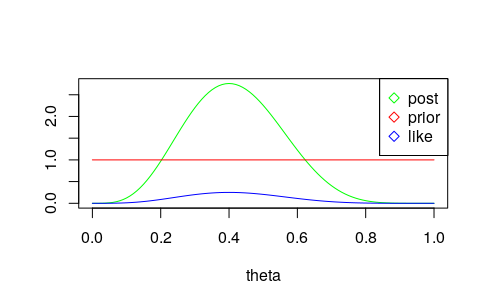
\includegraphics[width=100mm]{pics/Rplot}
\end{center}

\end{frame}
%----------------------------------------------------------------------------------------


\begin{frame}[fragile]
\frametitle{Binomial}

Finding a {\bf posterior/credible interval} is easy. Recall that $\theta \mid y \sim \text{Beta}(y+1, n-y+1)$


\begin{verbatim}
# find a posterior interval
left <- qbeta(.025, y+1, n-y+1)
right <- qbeta(.975, y+1, n-y+1)
cat("posterior interval", "(", left, ",", right, ")")
posterior interval ( 0.1674881 , 0.6920953 )
\end{verbatim}

Finding {\bf highest posterior density intervals} is a little trickier, but even more useful.
\end{frame}

%----------------------------------------------------------------------------------------


\begin{frame}[fragile]
\frametitle{Binomial prediction}

We just found $\theta \mid y \sim \text{Beta}(y+1, n-y+1)$. \\
What's the chance that $\tilde{y} = 1$ if $\tilde{y} \mid \theta \sim \text{Bern}(\theta)$?
\pause

\begin{align*}
\text{Pr}(\tilde{y}=1 \mid y) &= \int \text{Pr}(\tilde{y} =1 \mid \theta) p(\theta \mid y) \text{d}\theta \\
&= \int \theta p(\theta \mid y) \text{d}\theta \\
&= E[\theta \mid y] = (y+1)/(n+2)
\end{align*}


\end{frame}


%----------------------------------------------------------------------------------------


\begin{frame}[fragile]
\frametitle{Conjugacy}

\begin{block}{Conjugate Priors}
Let $\mathcal{F}$ be a class of sampling distributions $p(y \mid \theta)$. Let $\mathcal{P}$ be a class of prior distributions $p(\theta)$. Then $\mathcal{P}$ is {\bf conjugate} for $\mathcal{F}$ if 
\[
p(\theta \mid y) \in \mathcal{P}
\]
for all $p(\theta) \in \mathcal{P}$ and $p(y \mid \theta) \in \mathcal{F}$.
\end{block}

\end{frame}

%----------------------------------------------------------------------------------------

\begin{frame}[fragile]
\frametitle{Conjugacy example 1}

beta - binomial:
\begin{enumerate}
\item $p(\theta) = [\text{B}(\alpha,\beta)]^{-1} \theta^{\alpha-1}(1-\theta)^{\beta-1}$
\item $p(y \mid \theta) = \prod_i \theta^{y_i}(1-\theta)^{1-y_i} $
\item $p(\theta \mid y) \propto \theta^{\sum_i y_i}(1-\theta)^{n-\sum_i y_i}\theta^{\alpha-1}(1-\theta)^{\beta-1}$
\end{enumerate}

% so $\theta \mid y \sim \text{Beta}(\alpha + \sum_i y_i , \beta + n - \sum_i y_i)$, or

\[
p(\theta \mid y) = \frac{1}{\text{B}(\alpha + \sum_i y_i, \beta + n -
  \sum_i y_i)} \theta^{\alpha + \sum_i y_i - 1}(1-\theta)^{\beta +
  n-\sum_i y_i - 1}
\]

\end{frame}



%----------------------------------------------------------------------------------------

\begin{frame}[fragile]
\frametitle{Conjugacy example 2}


inverse gamma-normal (known mean):
\begin{enumerate}
\item $p(\sigma^2 ) \propto (\sigma^2)^{-(\alpha+1)} \exp\left( -\beta / \sigma^2 \right)$
\item $p(y \mid \sigma^2) \propto (\sigma^2)^{-n/2} \exp\left[-\frac{1}{2 \sigma^2} \sum_i \left(y_i - \theta \right)^2 \right] $
\item $p(\sigma^2 \mid y) = \text{Inverse-Gamma}\left(\alpha + \frac{n }{2}, \beta + \frac{  n v }{2} \right)$
\end{enumerate}
where $\theta$ is some known mean, and $v = \sum_i(y_i - \theta)^2 / n$.

\end{frame}


%----------------------------------------------------------------------------------------

\begin{frame}[fragile]
\frametitle{Conjugacy example 2}

Instead of $\alpha$ and $\beta$ as prior parameters, the book uses the transformed ones: $\alpha = \nu_0/2$ and $\beta = \nu_0 \sigma^2_0/2$
\begin{align*}
&p(\sigma^2 \mid y)\\
&\propto (\sigma^2)^{-(\nu_0/2+1)} \exp\left( - \frac{\sigma_0^2 \nu_0}{ 2\sigma^2} \right)(\sigma^2)^{-n/2} \exp\left[-\frac{1}{2 \sigma^2} \sum_i \left(y_i - \theta \right)^2 \right] \\
& \vdots \tag{homework} \\
&\propto (\sigma^2)^{-(\frac{n + \nu_0}{2}  +1)} \exp\left[-\frac{1}{2 \sigma^2}\left(\nu_0 \sigma^2_0 + n v  \right)  \right]
\end{align*}

\end{frame}

%----------------------------------------------------------------------------------------

\begin{frame}[fragile]
\frametitle{Conjugacy example 3}


gamma-Poisson:
\begin{enumerate}
\item $p(\theta) \propto \theta^{\alpha - 1}\exp\left( - \beta \theta \right)$
\item $p(y \mid \theta) \propto e^{-n\theta} \theta^{\sum_i y_i}$
\item $p(\theta \mid y)  = \text{Gamma}(\alpha + n\bar{y}, \beta + n)$
\end{enumerate}

note the rate parameterization
\end{frame}

%----------------------------------------------------------------------------------------

\begin{frame}[fragile]
\frametitle{Conjugacy example 3}


\begin{align*}
&p(\theta \mid y)\\
&\propto \theta^{\alpha - 1}\exp\left( - \beta \theta \right) \exp(-n\theta) \theta^{\sum_i y_i} \\
&\propto \theta^{\sum_i y_i + \alpha - 1}\exp\left( - (\beta +n)\theta \right)
\end{align*}

\end{frame}

%----------------------------------------------------------------------------------------

\begin{frame}[fragile]
\frametitle{Conjugacy example 4}


gamma-exponential:
\begin{enumerate}
\item $p(\theta) \propto \theta^{\alpha - 1}\exp\left( - \beta \theta \right)$
\item $p(y \mid \theta) \propto \theta^n  \exp\left(- \theta \sum_i y_i\right)$
\item $p(\theta \mid y)  = \text{Gamma}(\alpha + n, \beta + \sum_i y_i)$
\end{enumerate}


\end{frame}

%----------------------------------------------------------------------------------------

\begin{frame}[fragile]
\frametitle{Conjugacy example 5}


normal-normal (known variance):
\begin{enumerate}
\item $p(\theta) \propto \exp\left[-\frac{1}{2 \tau_0}(\theta - \mu_0)^2 \right]$
\item $p(y \mid \theta) \propto \prod_i \exp\left[-\frac{1}{2 \sigma^2} \left(y_i - \theta \right)^2 \right] $
\item $p(\theta \mid y) = \text{Normal}(\mu_n, \tau_n^2)$
\end{enumerate}


\end{frame}

%----------------------------------------------------------------------------------------

\begin{frame}[fragile]
\frametitle{Conjugacy example 5}

\begin{align*}
&p(\theta \mid y) \\
&\propto \exp\left[-\frac{1}{2 \tau_0^2}(\theta - \mu_0)^2 \right] \prod_i \exp\left[-\frac{1}{2 \sigma^2} \left(y_i - \theta \right)^2 \right] \\
&= \exp\left[-\frac{1}{2 \tau_0^2}(\theta - \mu_0)^2 \right] \exp\left[-\frac{1}{2 \sigma^2} \sum_i \left(y_i - \theta \right)^2 \right] \\
&\vdots \tag{homework} \\
&\propto \exp\left[ - \frac{1}{2 \tau_n^2} (\theta - \mu_n)^2 \right]
\end{align*}

where $\frac{1}{\tau_n^2} = \frac{n}{\sigma^2} + \frac{1}{\tau_0^2}$ and $\mu_n = \frac{ \mu_0 \sigma^2 + n \tau_0^2 \bar{y}}{n \tau_0^2 + \sigma^2} = \mu_0 \left( \frac{ 1/\tau_0^2 }{n / \sigma^2 + 1/ \tau_0^2}\right) + \bar{y} \left(\frac{ n /\sigma^2}{n /\sigma^2 + 1/\tau_0^2}\right)$. 

\end{frame}



%----------------------------------------------------------------------------------------

\begin{frame}[fragile]
\frametitle{Conjugacy example 6}

general exponential families:
\begin{enumerate}
\item $p(\theta) \propto g(\theta)^{\eta} \exp\left[\phi(\theta)' \nu \right]$
\item $p(y \mid \theta) \propto g(\theta)^{n} \exp\left[\phi(\theta)' t(y) \right] $
\item $p(\theta \mid y) \propto g(\theta)^{\eta + n} \exp\left[\phi(\theta)' \{t(y) + \nu\} \right] $
\end{enumerate}


\end{frame}

%----------------------------------------------------------------------------------------

\begin{frame}[fragile]
\frametitle{Improper/Proper Priors}

\begin{block}{Proper Prior}
A prior $p(\theta)$ is {\bf improper} if it integrates to $\infty$.
\end{block}

Improper priors may still be used, as long as the *posterior* integrates to $1$. If one is using an improper prior, one must check that 
\[
\int p(y \mid \theta) p(\theta) \text{d}\theta < \infty
\]
Interpretation should also be justified.


\end{frame}

%----------------------------------------------------------------------------------------

\begin{frame}[fragile]
\frametitle{Improper/Proper Priors example 1}

$p(\sigma^2) \propto (\sigma^2)^{-1}$ is a common example of an improper (and noninformative) prior:
\begin{align*}
&p(\sigma^2)  p(y \mid \sigma^2)\\
&\propto (\sigma^2)^{-1} (\sigma^2)^{-n/2}\exp\left[-\frac{1}{2 \sigma^2} \sum_i \left(y_i - \theta \right)^2 \right] \\
&= (\sigma^2)^{-[(n/2)+1]}\exp\left[-\frac{nv}{2 \sigma^2} \right]
\end{align*}
with $v = \sum_i(y_i - \theta)^2 / n$. So
\[
\sigma^2 \mid y \sim \text{Inv-Gamma}(n/2, nv/2)
\]


\end{frame}


% %----------------------------------------------------------------------------------------
% 
% \begin{frame}[fragile]
% \frametitle{Prior Lingo}
% 
% \begin{itemize}
% \item objective priors
% \item reference prior
% \item noninformative prior
% \item weakly informative prior
% \end{itemize}
% 
% 
% \end{frame}

%----------------------------------------------------------------------------------------

\begin{frame}[fragile]
\frametitle{Jeffreys' Prior}

Setting: we want $p(\theta)$ to be as noninformative as possible. Perhaps we don't have any pre-existing scientific knowledge about $\theta$. 
\newline

If you don't have any ``information" about $\theta$, then you also don't have any ``information" about $\phi = h(\theta)$ (1-to-1), right?
\newline
\pause

Uh oh:
\[
p(\phi) = p(\theta) \bigg\rvert \frac{\text{d}\theta}{\text{d}\phi } \bigg\rvert 
\]
$|h'(\theta)|^{-1}$ isn't always flat!

\end{frame}


%----------------------------------------------------------------------------------------

\begin{frame}[fragile]
\frametitle{Jeffreys' Prior}

Should we make $p(\theta)$ flat, or should we make $p(\phi)$ flat? Wouldn't it be nice if we had a rule to tell us? 
\newline


\begin{block}{Jeffreys Prior}
The Jeffreys' prior for $\theta$ is 
\[
p(\theta) \propto [J(\theta)]^{1/2}
\]
where $J(\theta)$ is the Fisher Information of one data point.
\end{block}

\end{frame}

%----------------------------------------------------------------------------------------

\begin{frame}[fragile]
\frametitle{Jeffreys' Prior}

You will show in your homework that 
\[
J(\phi) = J(\theta) \bigg\rvert \frac{\text{d}\theta}{ \text{d}\phi } \bigg\rvert^2
\]
so 
\[
p(\phi) = \sqrt{J(\phi)} = \sqrt{J(\theta)} \bigg\rvert \frac{\text{d}\theta}{ \text{d}\phi } \bigg\rvert = p(\theta) \bigg\rvert \frac{\text{d}\theta}{ \text{d}\phi } \bigg\rvert.
\]


No more ambiguity! If we find $p(\theta)$ first, then transform to $\phi$ to find $p(\phi)$, then that's the same as if we just found $p(\phi)$ straight away following Jeffreys' strategy. This prior is ``invariant to parameterization." 
\newline

Note that this does not mean that one parameterization is guaranteed to be flat, nor does it mean that the densities are the same functions.

\end{frame}

%----------------------------------------------------------------------------------------

\begin{frame}[fragile]
\frametitle{Jeffreys' Prior Example 1}

Example $p(y \mid \theta) = (2\pi)^{-1/2}  \theta^{-1/2} \exp\left[-\frac{1}{2\theta}y^2 \right]$. $J(\theta) = \frac{1}{\theta^2}$. 
\newline

So Jeffreys' prior is 
\[
\sqrt{J(\theta)} \propto 1/\theta
\]

If you define $\phi = \log \theta $ then

\[
p(\phi) = p_{\theta}( \theta[\phi]) \bigg\rvert \frac{\text{d} \theta[\phi]}{ \text{d} \phi} \bigg\rvert \propto e^{-\phi + \phi} = 1
\]

\end{frame}

%----------------------------------------------------------------------------------------

\begin{frame}[fragile]
\frametitle{Noninformative Priors}

Example $p(y \mid \theta) = \binom{n}{y} \theta^y (1-\theta)^{n-y}$. We fix a parameterization. 
\newline

\begin{enumerate}
\item Bayes'-Laplace: $p(\theta) \propto 1$
\item Jeffreys': $\sqrt{J(\theta)} \propto \theta^{1/2-1}(1-\theta)^{1/2-1}$
\item $p(\theta) \propto \theta^{0-1}(1-\theta)^{0-1}$ (if $p(\text{logit} \theta) \propto 1$)
\end{enumerate}

Hopefully our likelihood will stay away from those side peaks.


\begin{center}
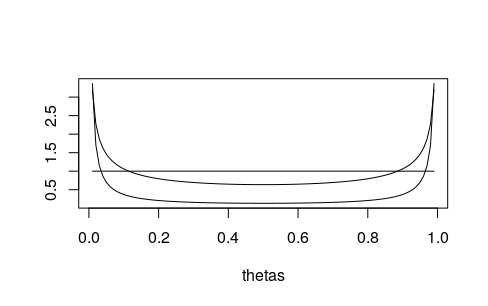
\includegraphics[width=80mm]{pics/Rplot2.png}
\end{center}


\end{frame}


\end{document} 


%%% Local Variables:
%%% mode: latex
%%% TeX-master: t
%%% End:
